\documentclass[11pt]{article}
\usepackage[T1]{fontenc}
\usepackage[utf8]{inputenc}
\usepackage[english,spanish,es-nodecimaldot]{babel}
\usepackage{lmodern}
\usepackage{microtype}
\usepackage{geometry}
\usepackage{amsmath,amssymb}
\usepackage{booktabs}
\usepackage{adjustbox}
\usepackage{csquotes}
\usepackage{caption}
\usepackage{graphicx}
\usepackage{xcolor}
\usepackage{setspace}
\usepackage[backend=biber,style=apa]{biblatex}
\DeclareLanguageMapping{spanish}{spanish-apa}
\usepackage[hidelinks]{hyperref}

\geometry{margin=1in}
\graphicspath{{figuras/}}
\setstretch{1.15}
\addbibresource{bibliografia-2-2.bib}


\newcommand{\note}[2]{%
  \par\vspace{0.5ex}
  \begin{minipage}{#1}\footnotesize\textit{Nota:} #2\end{minipage}%
}
% Marcador visible de puntos abiertos (buscar "PENDIENTE" antes de enviar)
\newcommand{\pendiente}[1]{{\color{red}\small[PENDIENTE: #1]}}

\title{Demanda Inversa y Formación del Precio \textit{Ex-Vessel} en la Pesquería de Pelágicos Menores de la Zona Centro-Sur de Chile\thanks{\acknowledgements}}
\author{
  Arnol Arche\\ {\itshape\large Universidad de Concepción\/}
  \and
  Ricardo Jara\\ {\itshape\large Universidad de Concepción\/}
}
\date{\today}
\def\acknowledgements{%
  Se agradece al profesor guía Felipe Quezada-Escalona por su apoyo y rigurosidad, y al financiamiento de la Agencia Nacional de Investigación y Desarrollo (ANID) a través del proyecto FONDECYT de Iniciación N\textsuperscript{o} 11250223. Se agradece también al Instituto de Fomento Pesquero (IFOP) por facilitar las bases de datos.
}
\hypersetup{
  pdftitle = {Demanda Inversa y Formación del Precio Ex-Vessel en la Pesquería de Pelágicos Menores de la Zona Centro-Sur de Chile},
  pdfauthor = {Arnol Arche, Ricardo Jara},
}


\begin{document}

% Title Page -------------------------------------------------------------------
\maketitle
\begin{abstract}
  \small
  Este trabajo estima la flexibilidad inversa del precio \textit{ex-vessel} del complejo sardina común--anchoveta en la zona centro-sur de Chile, con un panel planta-mes de la industria de reducción (427 observaciones, 16 plantas, 2012--2024) y el desembarque instrumentado con la biomasa de sardina y la cuota. La flexibilidad estimada es $-0{,}193$: un desembarque 10~\% mayor se asocia con un precio 1,9~\% menor. Los instrumentos son débiles y varían solo entre años, por lo que la inferencia es frágil: el intervalo de Anderson-Rubin es $[-0{,}605;\ -0{,}090]$, pero con \textit{wild bootstrap} por año no se rechaza $\gamma=0$ al 5~\% ($p=0{,}078$). El traspaso del precio internacional de la harina es parcial. El signo es estable y la magnitud, imprecisa.

  \smallskip\noindent\textit{Palabras clave:} demanda inversa, precio \textit{ex-vessel}, pesquerías pelágicas, variables instrumentales, instrumentos débiles. \textit{Clasificación JEL:} Q22, C26, D43.
\end{abstract}

\begin{otherlanguage}{english}
\begin{abstract}
  \small
  \noindent\textbf{Abstract.} In central-southern Chile, the volume of small pelagic fish reaching processing plants depends largely on biomass, climate and quota, yet little is known about how much the beach price falls when landings rise. This paper estimates that inverse price flexibility for the common sardine--anchoveta complex with a plant-month panel of the reduction industry (427 observations, 16 plants, 2012--2024), instrumenting landings with sardine biomass and the quota. The estimated flexibility is $-0.193$: a 10\% increase in landings is associated with a 1.9\% lower price. The instruments are weak and vary only across years, so inference is fragile: the Anderson-Rubin interval is $[-0.605,\,-0.090]$, but a year-cluster wild bootstrap does not reject $\gamma=0$ at 5\% ($p=0.078$). Pass-through of the international fishmeal price is partial. The sign is stable; the magnitude is imprecise.
\end{abstract}
\end{otherlanguage}
\newpage

% ------------------------------------------------------------------------------
\section{Introducción}\label{sec:intro}
% ------------------------------------------------------------------------------
En la zona centro-sur de Chile, la oferta de pelágicos menores llega a las plantas con un volumen que depende sobre todo de factores que el precio no controla. Las capturas de anchoveta (\textit{Engraulis ringens}), sardina común (\textit{Strangomera bentincki}) y jurel (\textit{Trachurus murphyi}) siguen las oscilaciones del ENSO, los ciclos de reclutamiento y los cambios de régimen de largo plazo \parencite{alheit2004, chavez2003}, y la perecibilidad y las restricciones regulatorias hacen que, dentro del mes, la cantidad desembarcada responda poco al precio del día \parencite{dresdner2014}. Cuando la oferta está en gran medida determinada de antemano, es el precio el que se ajusta, y la herramienta natural es la demanda inversa \parencite{anderson1980}, cuya estructura empírica para bienes perecibles desarrollaron \textcite{barten1989} y \textcite{eales1994}. Tratar el precio como exógeno en este contexto distorsiona la estimación de las rentas del sector \parencite{gordon2015}.

El precio de primera venta que pagan las plantas de reducción opera como una demanda derivada del mercado de harina de pescado \parencite{asche2002}, segunda línea de exportación del sector extractivo chileno (US\$~454,2 millones en 2024, con China como destino de 61,3~\% del volumen; \cite{SUBPESCA2025informe}), cuyo precio internacional determina sobre todo Perú. Las plantas tienen una capacidad de recepción fija en el corto plazo \parencite{dresdner2014} y son pocos compradores, de modo que el efecto del desembarque local sobre el precio de playa no es evidente, y es el efecto que importa para evaluar cuotas y rentas.

La demanda inversa se ha estimado para pesquerías del Golfo de México \parencite{beach2001, park2004}, de Nueva Inglaterra \parencite{lee2013}, de mercados europeos \parencite{klonaris2009, thong2012} y de subastas de atún \parencite{sun2017, sun2019}. Con identificación instrumental, el antecedente más cercano es \textcite{hammarlund2022wind}, que instrumenta la demanda de langosta noruega con variables meteorológicas; en Chile, \textcite{penatorres2017} muestran que las anomalías de temperatura superficial cambian la localización de la flota de jurel. Hasta donde alcanza la revisión de los autores, no se conoce una estimación con identificación instrumental para la pesquería de reducción de pelágicos menores del Pacífico suroriental, y cualquier modelo de optimización pesquera necesita la derivada del precio respecto del desembarque.

El objetivo es estimar la flexibilidad inversa $\gamma=\partial\ln p/\partial\ln h$ del precio \textit{ex-vessel} del complejo respecto del desembarque local y la derivada en niveles $\partial P/\partial h$, insumo para evaluar cuotas en un modelo bioeconómico de la pesquería. Se contrastan tres hipótesis: que el precio responde inversamente a la oferta local ($H_1$: $\gamma<0$); que el traspaso del precio FOB de la harina es imperfecto ($H_2$: $\beta<1$); y que el desembarque de jurel incide sobre el precio del complejo por competencia en capacidad de procesamiento ($H_3$: $\delta\neq0$). Para ello se usa un panel planta-mes de la industria de reducción (427 observaciones, 16 plantas y 111 meses entre febrero de 2012 y junio de 2024), con efectos fijos de planta y el desembarque instrumentado con la biomasa de sardina y la cuota. La flexibilidad estimada es $-0{,}193$, y un aumento de 10~\% en los desembarques se asocia con una caída de 1,9~\% en el precio. Como los instrumentos son débiles, la inferencia descansa en el intervalo de Anderson-Rubin, $[-0{,}605;\ -0{,}090]$, aunque con \textit{wild bootstrap} por año no se rechaza $\gamma=0$ al 5~\% ($p=0{,}078$). El traspaso del precio internacional es parcial, y excluir ocho observaciones anómalas de una planta en 2013 reduce la magnitud del coeficiente (con ellas es de $-0{,}357$) sin cambiar su signo.

El trabajo aporta una estimación de $\gamma$ con variables instrumentales en un panel planta-mes, con inferencia robusta a instrumentos débiles y con la sensibilidad a una anomalía de datos documentada; un diagnóstico de la identificación, que es interanual y proviene sobre todo de la biomasa evaluada (la cuota autorizada no tiene efecto significativo por separado sobre el precio); y los parámetros de política en niveles, con su intervalo y con una cota inferior de la elasticidad de la demanda derivada.
% ------------------------------------------------------------------------------
\section{Marco Teórico}\label{sec:theory}
% ------------------------------------------------------------------------------
\subsection{Demanda inversa y flexibilidad}\label{sec:inversa}

La demanda inversa invierte la relación marshalliana convencional: el precio se modela como función de cantidades predeterminadas \parencite{anderson1980}, y \textcite{eales1994} extendieron esa lógica al caso multiespecie. El parámetro central es la flexibilidad inversa $\gamma=\partial\ln p/\partial\ln h$, el cambio porcentual del precio ante un cambio de 1~\% en la cantidad desembarcada. Es una flexibilidad y no una elasticidad: su recíproco solo coincide con la elasticidad cuando no hay efectos cruzados \parencite{park1999}, y en general $1/|\gamma|$ es una cota inferior de la elasticidad en valor absoluto \parencite{houck1965}. La condición es que la oferta sea predeterminada respecto del precio contemporáneo, lo que en el horizonte mensual exige capacidad fija de las plantas y una cuota efectivamente restrictiva (\autoref{sec:interanual}). Como el volumen mensual agrega decisiones de varios días y los datos rechazan su exogeneidad (\autoref{sec:principal}), la predeterminación no se supone: se impone con instrumentos. La dirección del sesgo por simultaneidad depende del contexto: \textcite{hammarlund2022wind} documentan, para la langosta noruega, que instrumentar atenúa la estimación sin cambiar su signo.

\subsection{Demanda derivada, agregación y estructura del mercado}\label{sec:derivada}

El precio \textit{ex-vessel} es una demanda derivada: refleja lo que las plantas están dispuestas a pagar por la materia prima según el precio del producto transformado, una vez descontados los costos de procesamiento y los márgenes \parencite{asche2002}. En su versión fuerte, la Ley del Precio Único predice que el precio local se mueve proporcionalmente con el precio FOB \parencite{fackler2001}:
\begin{equation}\label{eq:lop}
  \ln p_{\text{ex-vessel}} = \alpha + \beta \ln P_{\text{FOB}} + \varepsilon,
\end{equation}
donde $\beta=1$ indica transmisión perfecta y $0<\beta<1$, integración imperfecta. La evidencia internacional rechaza la versión fuerte en el corto plazo \parencite{asche2007, nielsen2005whitefish, squires2023manta}, y aquí el FOB relevante lo determina sobre todo Perú, que concentra entre 26~\% y 34~\% de las exportaciones mundiales de harina \parencite{oecd_fao2023}. La literatura sectorial reporta una convención de precio de playa de entre 11 y 13~\% del FOB, referida al jurel \parencite{dresdner2014, kroetz2017}, que la \autoref{sec:fob} contrasta con la relación marginal entre ambos precios. Se espera, por tanto, un traspaso imperfecto del FOB ($H_2$).

Reducir el sistema multiespecie a una sola ecuación se apoya en el teorema de la mercancía compuesta \parencite{hicks1939, leontief1936}: si los precios relativos de un grupo de bienes se mantienen constantes, el grupo puede tratarse como un solo bien. La condición se cumple en el límite, porque sardina y anchoveta reciben precios idénticos en 90,4~\% de las observaciones en que una planta reporta ambas (\autoref{sec:data}), y $\gamma$ es la flexibilidad propia del bien compuesto. El jurel queda fuera del agregado y entra como control, porque puede presionar la capacidad de recepción de las plantas en los meses de abundancia conjunta ($H_3$).\label{sec:agregacion}

Dos mecanismos predicen $\gamma<0$ ($H_1$): el oligopsonio, en el que menos compradores deprimen el precio del insumo por debajo del valor marginal del producto \parencite{rubens2023}, y una capacidad de procesamiento cuasi fija en el corto plazo, que traslada el exceso de oferta al precio \parencite{dresdner2014}. El modelo reducido no los separa: $\gamma<0$ es condición necesaria pero no suficiente para poder de compra. El panel registra 11 plantas con datos en 2012 y una en 2024 (\autoref{fig:cobertura}), pero esa caída refleja la cobertura de reporte a IFOP y no mide concentración. En la dinámica, el oligopsonio implica una pendiente cada vez más negativa y la capacidad cuasi fija la mantiene estable, lo que se examina, con poco poder, en la \autoref{sec:robustez}.
% ------------------------------------------------------------------------------
\section{Datos}\label{sec:data}
% ------------------------------------------------------------------------------
\subsection{Fuentes y cobertura}

El estudio cubre la macrozona centro-sur de Chile (regiones de Valparaíso a Los Lagos) con frecuencia mensual, sobre un marco de 156 meses (enero de 2012 a diciembre de 2024) y una cobertura efectiva de 111 meses, de febrero de 2012 a junio de 2024; en promedio reportan 3,8 plantas por mes (mediana 4; mínimo 1; máximo 10). Los precios de primera venta y los desembarques industriales provienen de IFOP, los artesanales de SERNAPESCA, la biomasa acústica de sardina de las evaluaciones anuales de IFOP y el TAC del complejo de las resoluciones de SUBPESCA. El precio internacional de la harina de pescado (proteína 65~\%) y el FOB peruano, instrumento externo del FOB chileno, provienen de las series mensuales del Banco Central de Chile. Las variables oceanográficas por puerto (reanálisis GLORYS12V1) solo se usan en un escenario alternativo de instrumentos. Los precios, incluido el FOB, se expresan en pesos constantes de junio de 2024, deflactados con el IPC del INE.

\subsection{Panel planta-mes, complejo y anomalía de 2013}\label{sec:anomalia}

El panel cruza las hojas PRECIO y PROCESO del Monitoreo Económico de la Industria Pesquera y Acuícola Nacional de IFOP y retiene las plantas de línea ANIMAL o MIXTA\_AH de la macrozona con precio positivo. El filtro base entrega 497 observaciones planta-mes y 17 plantas; el cruce con PROCESO deja 435 y 16, porque la planta que sale (NUI 1916) tiene 33 meses de precio reportado y ningún desembarque. Se excluyen además ocho observaciones de la planta con NUI 90073 en 2013: sus precios del complejo, de 191.270 a 517.387 pesos nominales por tonelada, y los del jurel que reporta ese año son entre dos y cinco veces los de las otras plantas y ya están así en la fuente, lo que indica un artefacto de reporte y no un precio de mercado (\autoref{sec:appendix}). La muestra de estimación queda en 427 observaciones y 16 plantas. En la especificación principal, las ocho filas llevan el coeficiente a $-0{,}357$ (EE $0{,}116$; IC $[-0{,}586;\ -0{,}127]$) contra $-0{,}193$ sin ellas: casi el doble, sin cambio de signo ni de significancia (\autoref{tab:robustez}).

Sardina común y anchoveta reciben precios idénticos en 90,4~\% de las observaciones en que una misma planta reporta ambas en el mismo mes (208 de 230 casos); en los 22 restantes, la diferencia relativa tiene una mediana de 0,78~\% y una media de 18,76~\% en pesos nominales. Por eso se tratan como un complejo, con precio promedio ponderado por volumen y volumen igual a la suma de los desembarques industriales y artesanales, que las dos flotas venden a las mismas plantas. El jurel se registra aparte. Sobre las 427 observaciones, el precio \textit{ex-vessel} medio del complejo es de 162.543 pesos por tonelada, el desembarque medio de 69.122 toneladas y el FOB medio de 1.529.893 pesos por tonelada; el cociente entre precio y desembarque medios, $\bar P/\bar h=2{,}352$, fija el punto de evaluación de la derivada en niveles. La \autoref{tab:desc} del apéndice reporta las estadísticas del panel de 435 observaciones. La \autoref{fig:interanual} muestra que el precio real y el desembarque varían entre años y que el precio tiende a moverse en sentido contrario, aunque con ruido y con pocas plantas desde 2021.

\begin{figure}[htbp]
  \centering
  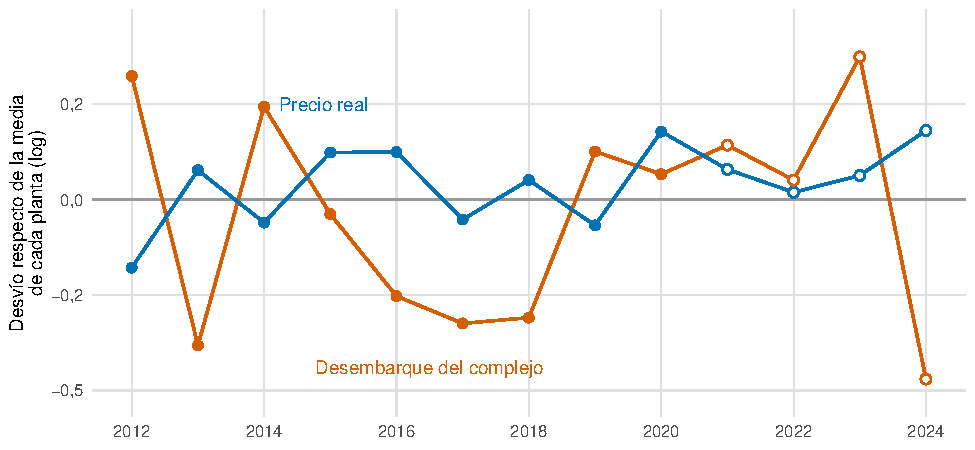
\includegraphics[width=0.9\textwidth]{fig_interanual.pdf}
  \caption{Precio real \textit{ex-vessel} y desembarque del complejo, promedios anuales}\label{fig:interanual}
  \note{0.9\textwidth}{Ambas series están en logaritmos, como desvío respecto de la media de cada planta. Los círculos huecos indican años con menos de 20 observaciones planta-mes. Fuente: elaboración propia con datos de IFOP y SERNAPESCA.}
\end{figure}
% ------------------------------------------------------------------------------
\section{Estrategia Empírica}\label{sec:strategy}
% ------------------------------------------------------------------------------
La especificación es una demanda inversa con efectos fijos de planta y variables instrumentales:
\begin{equation}\label{eq:iv}
  \ln p_{pt} = \alpha_p + \gamma \ln h_{t}^{\text{complejo}} + \beta \ln P_{\text{FOB},t}
              + \delta \ln h_{t}^{\text{jurel}} + \phi_1\,\mathrm{SEN}_t + \phi_2\,\mathrm{COS}_t
              + \lambda\, t + \varepsilon_{pt},
\end{equation}
donde $\ln p_{pt}$ es el precio real del complejo en la planta $p$ y el mes $t$, $h_t^{\text{complejo}}$ el desembarque macrozonal, $P_{\text{FOB},t}$ el precio internacional de la harina y $h_t^{\text{jurel}}$ el desembarque de jurel, que controla por la línea alternativa de procesamiento. Los armónicos estacionales $\mathrm{SEN}_t$ y $\mathrm{COS}_t$ aproximan el calendario de veda biológica fijado por la Subsecretaría de Pesca mediante decretos exentos anuales (p.\ ej.\ D.Ex.\ 51-2016 para la zona centro-sur), y $\lambda t$ es una tendencia lineal. Los efectos fijos $\alpha_p$ absorben la heterogeneidad permanente entre plantas, y los regresores de cantidad y precio externo no varían entre plantas dentro de un mes. El parámetro de interés es $\gamma$ ($H_1$), y los contrastes sobre $\beta$ ($H_2$) y $\delta$ ($H_3$) responden a las otras dos hipótesis. Como precio y cantidad se determinan simultáneamente, el desembarque es endógeno.

El desembarque se instrumenta con la biomasa acústica de sardina de la evaluación anual de IFOP y con el TAC anual de SUBPESCA. La biomasa proviene de métodos independientes del mercado de primera venta y el TAC es una resolución oficial fijada con base en evaluaciones de stock, por lo que se supone que ambos afectan el precio solo a través del volumen ofrecido; la exclusión es condicional a $\ln h^{\text{jurel}}$, que bloquea el canal clima $\rightarrow$ talla del jurel $\rightarrow$ destino a reducción $\rightarrow$ competencia por capacidad. Se comparan tres configuraciones alternativas como sensibilidad (los cuatro instrumentos originales, que agregan salinidad y temperatura superficial rezagada; solo el TAC; y los dos anuales con vedas; \autoref{tab:escenarios_instrumentos}). Como ambos instrumentos varían solo entre años, la identificación es interanual (\autoref{sec:interanual}).

La matriz de varianzas principal es la de Driscoll-Kraay \parencite{driscoll1998} con ancho de banda 4. Como el regresor de interés no varía dentro del mes, agrupar por planta ignora la dependencia relevante entre plantas del mismo mes, y las demás matrices (por planta, por mes, de dos vías, con ancho de banda 12, por año y por planta y año) se reportan como robustez (\autoref{tab:vcov}). La fortaleza de los instrumentos se evalúa con el $F$ efectivo de Montiel Olea-Pflueger \parencite{olea2013robust}, contra su valor crítico (19,7 para una distorsión máxima de 10~\% en el tamaño de un test de Wald de 5~\%, y 10,8 para una de 25~\%); el estadístico de Kleibergen-Paap se reporta solo como referencia. Como el $F$ efectivo queda por debajo del umbral, el intervalo para $\gamma$ es el de Anderson-Rubin, calculado por búsqueda en grilla sobre $\gamma_0\in[-2,2]$ con paso 0,005, que no depende de la fortaleza de la primera etapa; el estimador puntual (Driscoll-Kraay) y el intervalo provienen, por tanto, de procedimientos distintos.

El precio FOB se trata como exógeno al precio local porque Chile no mueve el mercado mundial de harina, y esto se contrasta con la función de control de \textcite{riversvuong1988}: se instrumenta el FOB chileno con el FOB peruano, que se supone excluible de la ecuación local, y se agrega el residuo $\hat v_{\text{FOB}}$ a la ecuación principal. Que el test no rechace no establece la exogeneidad. La robustez cubre la anomalía de 2013, las configuraciones de instrumentos, siete tratamientos del control de jurel, efectos fijos de año, la partición pre y post 2020 y una versión ponderada por materia prima procesada.
% ------------------------------------------------------------------------------
\section{Resultados}\label{sec:results}
% ------------------------------------------------------------------------------

\subsection{Resultado principal}\label{sec:principal}

El coeficiente principal es $\hat\gamma=-0{,}193$ (EE Driscoll-Kraay $0{,}0738$; $p=0{,}009$), sobre 427 observaciones, 16 plantas y 111 meses (\autoref{tab:principal}): un aumento de 10~\% en el desembarque del complejo se asocia con una caída de 1,9~\% en el precio. Como los instrumentos son débiles ($F$ efectivo de $7{,}27$, bajo el umbral de $19{,}7$), el intervalo de referencia es el de Anderson-Rubin, $[-0{,}605;\ -0{,}090]$, que excluye el cero; el de Wald queda como referencia. El $J$ de Hansen robusto no rechaza la sobreidentificación ($J=0{,}418$; $p=0{,}518$), aunque con instrumentos débiles su poder es bajo. La estimación por MCO da $-0{,}025$, una atenuación de unas ocho veces y no una inversión del signo, y el test de Wu-Hausman rechaza la exogeneidad del desembarque ($F=19{,}59$; $p=1{,}2\times10^{-5}$).

\begin{table}[htbp]
  \caption{Especificación principal, inferencia y diagnósticos}\label{tab:principal}
  \centering
  \small
  \begin{tabular}{@{} lcc @{}}
    \toprule
    Estadístico & Valor & $p$ o umbral \\
    \midrule
    $\hat\gamma$ ($\ln h_{\text{complejo}}$, instrumentada) & $-0{,}193$ & $0{,}009$ \\
    EE Driscoll-Kraay ($bw=4$) & $0{,}0738$ & --- \\
    IC 95~\% Driscoll-Kraay (Wald, referencia) & $[-0{,}338;\ -0{,}049]$ & --- \\
    \textbf{IC 95~\% Anderson-Rubin} & $\mathbf{[-0{,}605;\ -0{,}090]}$ & --- \\
    $F$ de Anderson-Rubin ($H_0:\gamma=0$) & $10{,}96$ & $<0{,}001$ \\
    $F$ efectivo de Olea-Pflueger & $7{,}27$ & umbral $\approx 19{,}7$ \\
    $F$ de Kleibergen-Paap (referencia) & $7{,}57$ & --- \\
    $J$ de Hansen robusto (Driscoll-Kraay) & $0{,}418$ & $0{,}518$ \\
    Wu-Hausman (exogeneidad del desembarque) & $F=19{,}59$ & $1{,}2\times10^{-5}$ \\
    $\hat\beta_{\text{FOB}}$ & $+0{,}388$ (EE $0{,}164$) & $0{,}019$ \\
    Wald $H_0:\beta_{\text{FOB}}=1$ & $t=-3{,}73$ & $0{,}0002$ \\
    Hausman del FOB ($\theta$ sobre $\hat v_{\text{FOB}}$) & $-0{,}105$ & $0{,}747$ \\
    $\hat\delta$ (desembarque de jurel) & $-0{,}032$ & $0{,}021$ \\
    $\hat\gamma$ por MCO, misma muestra & $-0{,}025$ & --- \\
    \bottomrule
  \end{tabular}
  \note{0.9\textwidth}{$N=427$, $G=16$ plantas, $T=111$ meses. Efectos fijos de planta, armónicos estacionales y tendencia lineal. Instrumentos: biomasa de sardina y TAC del complejo. El $J$ de Hansen tiene 1 grado de libertad (dos instrumentos, una endógena); el $J$ de Sargan clásico es $1{,}05$ ($p=0{,}305$). Con instrumentos débiles el intervalo de Wald no es válido como cobertura y el de Anderson-Rubin sí.}
\end{table}

\subsection{Primera etapa e identificación}\label{sec:interanual}

Ambos instrumentos tienen el signo esperado y son significativos (\autoref{tab:primera_etapa}). La identificación es interanual: los dos instrumentos explican 98,6~\% del $R^2$ \textit{within} de la primera etapa, y con efectos fijos de año quedan absorbidos y el modelo no está identificado (la corrida numérica da $\hat\gamma=0{,}008$, con $F=1{,}93$, y no se interpreta). Así, $\hat\gamma$ mide ajuste entre años y descansa en 111 meses de variación y no en 427 observaciones; al excluir cada año por separado queda entre $-0{,}279$ y $-0{,}155$. Los instrumentos oceanográficos por puerto no suman poder ($F$ conjunto $0{,}16$; $p=0{,}86$) y duplican el ancho del intervalo de Anderson-Rubin ($[-1{,}30;\ -0{,}09]$). La forma reducida muestra que la identificación proviene sobre todo de la biomasa (coeficiente sobre el precio de $-0{,}125$; EE $0{,}031$; $p<0{,}001$), mientras que el del TAC ($-0{,}098$; EE $0{,}066$; $p=0{,}145$) no se distingue de cero: el TAC aporta a la primera etapa, pero no tiene efecto significativo por separado sobre el precio.

La cuota es restrictiva en la mayoría de los años: la razón entre desembarque industrial y TAC es de al menos 85~\% en 11 de los 13 años, con mediana de 100,2~\% (101,0~\% con totales de industrial más artesanal; \autoref{tab:tac_razon}), y los años holgados son 2013 y 2024. Restringida a los años con cuota restrictiva, la estimación es $-0{,}144$ (EE $0{,}108$), con un intervalo que incluye el cero, y los años holgados (38 observaciones, 35 efectivas) no identifican el parámetro ($F=0{,}32$ en la primera etapa de la interacción). El test de igualdad entre regímenes no rechaza ($p=0{,}732$), pero con ese poder no discrimina: no prueba que $\gamma$ sea invariante a la restrictividad de la cuota.

\subsection{Inferencia y robustez}\label{sec:robustez}

Las otras seis matrices de varianza (por planta, por mes, de dos vías, con ancho de banda 12, por año y por planta y año) coinciden en el punto y rechazan la nula al 5~\% (\autoref{tab:vcov}), y el error estándar de Driscoll-Kraay es estable entre anchos de banda de 2 y 12 (de $0{,}067$ a $0{,}074$). El intervalo de Anderson-Rubin con cluster por año, $[-0{,}480;\ -0{,}120]$, es más estrecho que el de Driscoll-Kraay, que se mantiene como referencia por ser el más conservador. Con \textit{wild bootstrap} por año bajo la nula \parencite{cameron2008}, el valor $p$ de $\gamma=0$ es $0{,}078$: se rechaza al 10~\% y no al 5~\%, y el intervalo llega al borde de la grilla ($-1{,}5$) sin cerrarse.

La magnitud se mantiene cerca de $-0{,}19$ sin las ocho filas anómalas ($-0{,}192$ con cuatro instrumentos), en el núcleo de plantas con al menos 30 observaciones ($-0{,}201$) y con el filtro estricto de línea ANIMAL ($-0{,}182$; $p=0{,}055$); con las ocho filas aparece $-0{,}343$, incluso con el filtro quirúrgico ($-0{,}338$), que no las identifica porque en seis de los ocho meses la materia prima de línea ANIMAL supera con holgura a la de línea HUMANO. La \autoref{tab:robustez} del apéndice reporta todas las variantes.

El control de jurel tiene un coeficiente de $-0{,}032$ ($p=0{,}021$), pero no fue posible construir un test utilizable de su exogeneidad: el TAC del jurel es anual y la tendencia lineal absorbe su varianza. Bajo siete tratamientos del control, $\hat\gamma$ se mantiene entre $-0{,}178$ y $-0{,}199$ (\autoref{tab:jurel_tratamientos}). Con ello $H_3$ tiene apoyo débil: $\hat\delta$ difiere de cero solo en la especificación contemporánea, con el jurel instrumentado los coeficientes no son significativos ($-0{,}137$, $p=0{,}58$; $+0{,}066$, $p=0{,}16$) y los rezagos son nulos, por lo que se lee como asociación condicional y no como efecto causal.

Por período, $\hat\gamma=-0{,}218$ antes de 2020 ($n=352$; $p=0{,}014$) y $-0{,}020$ después ($n=75$; $p=0{,}786$), casi el valor por MCO ($-0{,}025$), como ocurre con un IV débil. La interacción ($+0{,}092$; $p=0{,}729$) no rechaza igualdad, de modo que el contraste no discrimina entre oligopsonio y capacidad cuasi fija.

\subsection{Traspaso del precio FOB}\label{sec:fob}

El FOB entra con $\hat\beta_{\text{FOB}}=0{,}388$ (EE $0{,}164$; $p=0{,}019$), y se rechaza la transmisión perfecta ($t=-3{,}73$; $p=0{,}0002$). La relación bivariada da $0{,}64$ en el panel y $0{,}53$ en la serie agregada mensual (\autoref{tab:fob_biv}). El cociente de medias $\bar P/\bar P_{\text{FOB}}=162.543/1.529.893=0{,}106$ queda algo bajo el rango convencional de 11 a 13~\%, y la muestra rechaza además la constancia de esa proporción: como $\beta<1$, el cociente $p/P_{\text{FOB}}$ disminuye cuando sube el precio internacional. Para contrastar la exogeneidad del FOB chileno se usó el FOB peruano: la primera etapa da $0{,}932$ ($t=11{,}06$; $R^2_{\text{within}}=0{,}779$) y el coeficiente de la función de control es $-0{,}105$ ($p=0{,}747$ con Driscoll-Kraay), por lo que no se rechaza la exogeneidad. En esa regresión $\hat\gamma=-0{,}183$ ($p=0{,}042$) y $\hat\beta_{\text{FOB}}=0{,}423$, frente a $0{,}542$ por MCO.

\subsection{Magnitudes en niveles}\label{sec:niveles}

En las medias de la \autoref{sec:data}, la derivada es $\partial P/\partial h=\hat\gamma\cdot\bar P/\bar h=-0{,}193\times2{,}352\approx-0{,}45$ CLP por tonelada en pesos de junio de 2024, con un rango de $-1{,}42$ a $-0{,}21$ sobre el intervalo de Anderson-Rubin. La versión ponderada por materia prima ($\hat\gamma=-0{,}0862$; EE $0{,}0353$; $p=0{,}016$) da $-0{,}20$ y se reporta como referencia, sin $F$ efectivo ni intervalo de Anderson-Rubin; es la pendiente de la tonelada representativa y no de la planta representativa. Por la desigualdad de Houck \parencite{houck1965}, $|e|\geq1/|\hat\gamma|=5{,}18$, y entre $1{,}65$ y $11{,}11$ sobre el intervalo; es una cota y no una estimación.

Encadenando $\hat\gamma$ con el coeficiente del TAC, $0{,}698\times(-0{,}193)=-0{,}135$ (EE delta $0{,}072$; intervalo de $[-0{,}304;\ -0{,}017]$ por Monte Carlo y de $[-0{,}276;\ +0{,}007]$ por el método delta, que supone independencia entre ambas estimaciones): una reducción de 10~\% en el TAC baja el desembarque en $7{,}09$~\%, sube el precio en $1{,}43$~\% (entre 0,2~\% y 3,3~\% por Monte Carlo) y reduce el ingreso bruto en $5{,}76$~\%, siempre que la cuota sea restrictiva. La forma reducida del TAC ($-0{,}098$; $p=0{,}145$) es menor que ese producto y no se distingue de cero, por lo que el efecto sobre el precio debe leerse con cautela; el efecto sobre el ingreso descansa sobre todo en la caída del desembarque. La conclusión de política se enuncia sobre el intervalo de Anderson-Rubin: todo valor cumple $|f|<1$, de modo que el ingreso bruto cae cuando baja la cuota, y todo valor implica $|e|>1{,}65$; el \textit{bootstrap} por año, que no cierra el intervalo, no garantiza esa condición.

% ------------------------------------------------------------------------------
\section{Discusión y conclusiones}\label{sec:discusion}
% ------------------------------------------------------------------------------

El precio \textit{ex-vessel} del complejo sardina--anchoveta responde a la oferta local con una flexibilidad negativa cercana a $-0{,}19$, y el signo se mantiene en las variantes de muestra, inferencia e instrumentos, salvo con efectos fijos de año, donde el modelo no está identificado. El traspaso del precio internacional es parcial: el cociente promedio entre ambos precios ($0{,}106$) es algo menor que la convención de 11 a 13~\% y cae cuando sube el FOB, de modo que la demanda derivada de las plantas no está perfectamente integrada al mercado internacional. Los datos no distinguen entre oligopsonio y capacidad cuasi fija (\autoref{sec:agregacion}), y la identificación proviene sobre todo de la biomasa evaluada, pues la cuota autorizada no tiene efecto significativo por separado sobre el precio.

En síntesis, $H_1$ tiene apoyo moderado: $\gamma<0$ según el intervalo de Anderson-Rubin, pero no al 5~\% con \textit{bootstrap} por año; $H_2$ se sostiene, con un traspaso de $0{,}388$; y $H_3$ tiene apoyo débil. Para la política, lo que el trabajo sostiene es una dirección y un orden de magnitud: bajar la cuota reduce el ingreso bruto de la flota si $|\gamma|<1$, y la magnitud se conoce con poca precisión (\autoref{sec:niveles}).

\subsection{Limitaciones}\label{sec:limitaciones}

Las limitaciones principales son de identificación. Los instrumentos son débiles, por lo que el estimador puntual es solo de referencia, y varían solo entre años: el parámetro mide ajuste entre años y no dentro del año, y con 13 años la inferencia asintótica es frágil. Los errores estándar con ancho de banda 12, por año y por planta y año son similares a los de Driscoll-Kraay, pero con \textit{wild bootstrap} por año $\gamma=0$ no se rechaza al 5~\% y el intervalo no se cierra por la izquierda. Como la identificación descansa sobre todo en la biomasa, la exclusión exige que esta no afecte el precio por otros canales, como la talla o la calidad del recurso. La razón desembarque/TAC supera 100~\% en varios años (\autoref{tab:tac_razon}), de modo que el TAC usado puede incluir cuotas suplementarias y saldos acumulados; si esas modificaciones responden al mercado, no sería exógeno. La serie de TAC se usa tal como está disponible, y distinguir el decreto inicial del modificado queda para una versión posterior. La magnitud depende de excluir ocho observaciones de una planta en 2013 (\autoref{sec:anomalia}), y la exogeneidad del control de jurel no pudo contrastarse.

Hay además limitaciones de alcance. El panel es desbalanceado: 45 de los 156 meses del marco no tienen reporte y, en los 111 restantes, la mediana es de cuatro plantas. El modelo es estático, y uno de corrección de errores \parencite{klonaris2009} permitiría separar la transmisión de corto y largo plazo del FOB. La exclusión del FOB peruano de la ecuación de precio local es un supuesto, la muestra posterior a 2020 es pequeña, y el diseño reducido no distingue oligopsonio de capacidad cuasi fija; hacerlo requiere información de costos marginales y márgenes a lo largo de la cadena de valor.

% ------------------------------------------------------------------------------
\newpage\printbibliography
% ------------------------------------------------------------------------------

% ------------------------------------------------------------------------------
\newpage\appendix
\section{Resultados Adicionales}\label{sec:appendix}
% ------------------------------------------------------------------------------

La planta con NUI 90073 reporta en 2013 precios del complejo de 191.270 a 517.387 pesos nominales por tonelada, contra el rango 87.500--206.286 de las otras ocho plantas activas. Los precios ya están así en la fuente, y en diciembre de 2013 la misma planta reporta jurel a 492.418 pesos por tonelada, cuando en 2012 lo reportaba entre 140.000 y 150.000: todo lo que informa ese año está inflado, especie por especie.

\begin{table}[htbp]
  \caption{Robustez y sensibilidad de $\hat\gamma$}\label{tab:robustez}
  \centering
  \begin{adjustbox}{max width=\textwidth,center}
    \begin{tabular}{@{} lcccccc @{}}
      \toprule
      Especificación & $N$ & $G$ & $\hat\gamma$ & EE & $p$ & IC 95~\% \\
      \midrule
      \textbf{Principal (dos instrumentos, DK)} & \textbf{427} & \textbf{16} & $\mathbf{-0{,}193}$ & $0{,}0738$ & $0{,}009$ & $[-0{,}338;\ -0{,}049]$ \\
      \midrule
      \multicolumn{7}{@{}l}{\textit{Sensibilidad a la anomalía (cuatro instrumentos, cluster por planta)}} \\
      A. Muestra completa (8 obs.\ de 90073 dentro) & 418 & 15 & $-0{,}343$ & $0{,}142$ & $0{,}030$ & $[-0{,}648;\ -0{,}039]$ \\
      B. Estricto: solo línea ANIMAL & 260 & 11 & $-0{,}182$ & $0{,}084$ & $0{,}055$ & $[-0{,}370;\ +0{,}005]$ \\
      C. Quirúrgico (ANIMAL $>$ HUMANO) & 401 & 15 & $-0{,}338$ & $0{,}134$ & $0{,}024$ & $[-0{,}625;\ -0{,}052]$ \\
      D. Núcleo: plantas con $\geq 30$ obs. & 293 & 6 & $-0{,}201$ & $0{,}056$ & $0{,}016$ & $[-0{,}340;\ -0{,}062]$ \\
      E. Sin las 8 obs.\ anómalas & 410 & 15 & $-0{,}192$ & $0{,}065$ & $0{,}011$ & $[-0{,}331;\ -0{,}052]$ \\
      \midrule
      \multicolumn{7}{@{}l}{\textit{Otras especificaciones sobre la muestra final}} \\
      Ponderada por materia prima & 427 & 16 & $-0{,}0862$ & $0{,}0353$ & $0{,}016$ & --- \\
      Principal con las 8 obs.\ de 90073 & 435 & 16 & $-0{,}357$ & $0{,}116$ & $0{,}002$ & $[-0{,}586;\ -0{,}127]$ \\
      Solo años con cuota restrictiva ($\geq 85$~\%) & 389 & --- & $-0{,}144$ & $0{,}108$ & $0{,}182$ & $[-0{,}358;\ +0{,}069]$ \\
      Efectos fijos de año (no identificado) & --- & --- & \multicolumn{4}{c}{instrumentos anuales absorbidos; $F=1{,}93$} \\
      \bottomrule
    \end{tabular}
  \end{adjustbox}
  \note{0.95\textwidth}{Las filas A--E usan los cuatro instrumentos originales (biomasa, TAC, salinidad y SST rezagada) con cluster por planta, sobre la muestra con filtro de SST (410--418 observaciones); el $F$ de Kleibergen-Paap es $44{,}19$, $61{,}91$, $51{,}75$ y $42{,}75$ en A, B, C y E. El núcleo (D) tiene solo seis conglomerados y una matriz de varianzas de rango 5, por lo que es una fila de robustez y no evidencia independiente de fortaleza. En la fila de años con cuota restrictiva el $p$ se calcula a partir del error estándar; sus 389 observaciones y las 38 de los años holgados suman 427. Las configuraciones alternativas de instrumentos están en la \autoref{tab:escenarios_instrumentos} y los tratamientos del jurel en la \autoref{tab:jurel_tratamientos}.}
\end{table}

\begin{figure}[htbp]
  \centering
  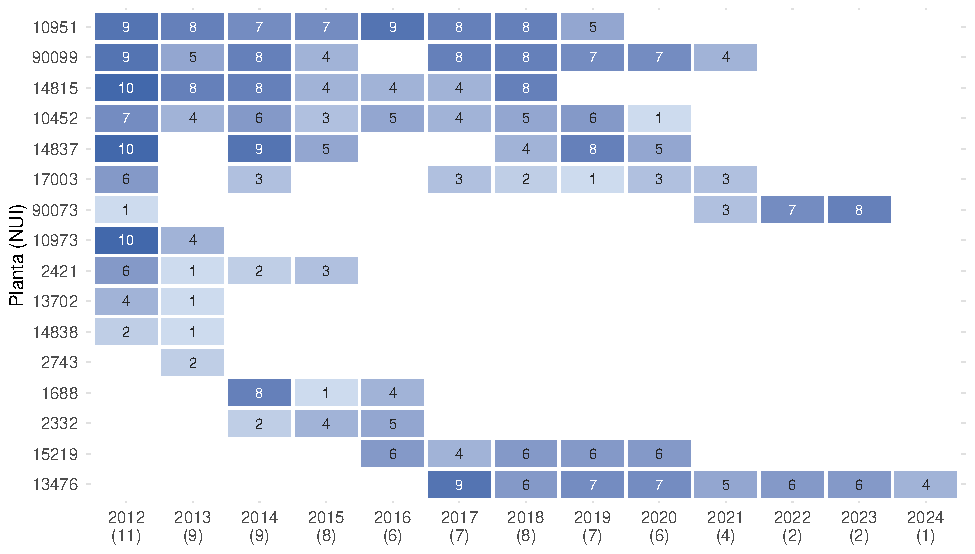
\includegraphics[width=\textwidth]{fig_cobertura.pdf}
  \caption{Cobertura del panel: observaciones planta-mes por planta y año}\label{fig:cobertura}
  \note{0.9\textwidth}{Muestra de estimación (427 observaciones, 16 plantas). Cada celda indica el número de meses observados; entre paréntesis, bajo cada año, el número de plantas con al menos una observación. Marco potencial: 156 meses; cobertura efectiva: 111 meses (febrero de 2012 a junio de 2024). Fuente: elaboración propia con datos de IFOP, 2012--2024.}
\end{figure}

\begin{table}[htbp]
  \caption{Razón entre desembarque y TAC del complejo centro-sur, 2012--2024}\label{tab:tac_razon}
  \centering
  \begin{tabular}{@{} lrrrl @{}}
    \toprule
    Año & Desembarque (miles t) & TAC (miles t) & Razón (\%) & Clasificación \\
    \midrule
    2012 & 921 & 1.041 & 88,4  & Restrictiva \\
    2013 & 275 &   660 & 41,8  & Holgada \\
    2014 & 599 &   547 & 109,5 & Restrictiva \\
    2015 & 496 &   454 & 109,3 & Restrictiva \\
    2016 & 352 &   360 & 97,6  & Restrictiva \\
    2017 & 396 &   389 & 101,7 & Restrictiva \\
    2018 & 401 &   313 & 128,1 & Restrictiva \\
    2019 & 472 &   471 & 100,2 & Restrictiva \\
    2020 & 427 &   491 & 86,9  & Restrictiva \\
    2021 & 514 &   559 & 91,9  & Restrictiva \\
    2022 & 439 &   426 & 103,0 & Restrictiva \\
    2023 & 605 &   334 & 180,8 & Restrictiva \\
    2024 & 248 &   352 & 70,5  & Holgada \\
    \midrule
    Mediana & & & 100,2 & 11 de 13 años $\geq 85$~\% \\
    \bottomrule
  \end{tabular}
  \note{0.9\textwidth}{Desembarque industrial de la línea ANIMAL (hoja PROCESO de IFOP), regiones V a X y XIV a XVI. TAC del complejo: industrial V--X más artesanal centro-sur, sin fauna acompañante, cesiones, consumo humano, investigación, imprevisto ni línea de mano. Las razones sobre 100~\% reflejan cuotas suplementarias, saldos no capturados traspasados de un año a otro y fauna acompañante contabilizada aparte. La razón con numerador y denominador totales (industrial más artesanal) da una mediana de 101,0~\% y las mismas conclusiones. La serie de TAC se usa tal como está disponible; su revisión queda para una versión posterior. Fuente: elaboración propia con datos de SUBPESCA e IFOP.}
\end{table}

\begin{table}[htbp]
  \caption{Robustez del titular bajo siete tratamientos del control de jurel}\label{tab:jurel_tratamientos}
  \centering
  \begin{tabular}{@{} lcc @{}}
    \toprule
    Tratamiento del jurel en \eqref{eq:iv} & $\hat\gamma$ & Coeficiente del jurel \\
    \midrule
    Contemporáneo (principal)                            & $-0{,}193$ & $-0{,}032$ ($p = 0{,}021$) \\
    Instrumentado con TAC jurel, con tendencia           & $-0{,}178$ & $-0{,}137$ ($p = 0{,}58$)   \\
    Instrumentado con TAC jurel, sin tendencia           & $-0{,}199$ & $+0{,}066$ ($p = 0{,}16$)   \\
    Rezagado $L1$ solamente                               & $-0{,}193$ & $-0{,}0023$ ($p = 0{,}84$) \\
    Contemporáneo $+$ $L1$                                & $-0{,}193$ & $L1$ en $-0{,}0006$ ($p = 0{,}96$) \\
    $L1 + L2$                                             & $-0{,}190$ & ninguno significativo       \\
    Sin control de jurel                                 & $-0{,}193$ & ---                         \\
    \bottomrule
  \end{tabular}
  \note{0.9\textwidth}{El resultado principal $\hat\gamma$ varía entre $-0{,}178$ y $-0{,}199$ bajo siete tratamientos alternativos del control de jurel, incluyendo exclusión completa. No existe un test de Hausman utilizable: el TAC del jurel es anual y el desembarque de jurel es estacional (mediana $63.300$ t en enero contra $400$ t en agosto), por lo que la primera etapa del instrumento es dominada por tendencia o colapsa cuando se incluye el término lineal. La robustez de $\hat\gamma$ a estos siete tratamientos vale como diagnóstico más fuerte que un test de exogeneidad que no rechace. Especificación principal: Driscoll-Kraay $bw=4$, $N=427$, $G=16$ plantas, muestra corregida.}
\end{table}

\begin{table}[htbp]
  \caption{Comparativa de escenarios de instrumentos sobre el titular}\label{tab:escenarios_instrumentos}
  \centering
  \begin{tabular}{@{} lcccl @{}}
    \toprule
    Instrumentos & $K$ & $F$ efectivo OP & IC Anderson-Rubin & Sargan $p$ \\
    \midrule
    Los cuatro originales (biomasa, TAC, SO, SST\_L1) & 4 & $3{,}59$ & $[-1{,}30;\ -0{,}09]$ & $0{,}66$ \\
    \textbf{Los dos anuales (biomasa, TAC)}           & 2 & $7{,}27$ & $[-0{,}605;\ -0{,}090]$ & $0{,}31$ \\
    Sólo TAC                                           & 1 & $8{,}24$ & $[-0{,}71;\ +0{,}02]$   & ---      \\
    Dos anuales $+$ vedas                              & 4 & $8{,}26$ & vacío (rechazo global)   & $0{,}003$ \\
    \bottomrule
  \end{tabular}
  \note{0.9\textwidth}{Matriz Driscoll-Kraay $bw=4$ en los cuatro escenarios. La columna Sargan reporta el $J$ clásico en los cuatro escenarios, para que sean comparables; en la configuración principal el $J$ de Hansen robusto bajo Driscoll-Kraay es $0{,}418$ ($p=0{,}518$; \autoref{tab:principal}). La configuración principal (dos anuales) se justifica en la \autoref{sec:strategy} por el canal estructural biomasa--cuota; las otras se reportan como sensibilidad. Los cuatro instrumentos originales mantienen el signo, pero amplían el intervalo de Anderson-Rubin por la debilidad conjunta ($F$ efectivo $3{,}59$); con sólo el TAC el intervalo incluye cero; y las vedas como instrumento adicional son rechazadas por Sargan ($p=0{,}003$) y entregan un conjunto AR vacío, lo que indica que los instrumentos no son mutuamente consistentes. El par anual \{biomasa, TAC\} combina la justificación económica, una sobreidentificación no rechazada (Sargan clásico $p=0{,}31$) y un intervalo acotado.}
\end{table}


\begin{table}[htbp]
  \caption{Estadísticas descriptivas de las variables principales}\label{tab:desc}
  \centering
  \begin{adjustbox}{max width=\textwidth,center}
    \begin{tabular}{@{} lrrrrrr @{}}
      \toprule
      Variable & $N$ & Media & DE & Mín & Mediana & Máx \\
      \midrule
      \multicolumn{7}{@{}l}{\textit{Panel A: Precios ex-vessel (CLP/ton, reales jun-2024)}} \\
      Sardina                 & 463 & 201.465 & 193.908 & 13.253 & 160.952 & 1.465.719 \\
      Anchoveta                & 253 & 217.676 & 260.832 & 82.359 & 160.294 & 1.621.613 \\
      Complejo                & 435 & 169.629 &  69.051 & 13.253 & 159.865 &   842.943 \\
      \midrule
      \multicolumn{7}{@{}l}{\textit{Panel B: Variables independientes básicas}} \\
      Desembarque complejo (ton) & 435 &  68.467 &  62.465 &    137 &  43.913 &   253.726 \\
      Precio FOB harina (CLP/ton, reales) & 435 & 1.527.895 & 239.474 & 1.020.305 & 1.468.923 & 2.256.749 \\
      \bottomrule
    \end{tabular}
  \end{adjustbox}
  \note{0.85\textwidth}{Estadísticas sobre las 435 observaciones del panel previo a excluir las ocho filas anómalas (la estimación usa 427). Los $N$ de sardina y anchoveta exceden 435 porque salen del filtro base, sin el cruce con PROCESO. Precios en pesos reales de junio de 2024. El complejo es un promedio ponderado por volumen. El punto de evaluación de la derivada en niveles usa las medias de las 427 observaciones de estimación (\autoref{sec:data}). Fuente: elaboración propia con datos de IFOP, 2012--2024.}
\end{table}

\begin{table}[htbp]
  \caption{Primera etapa del desembarque del complejo}\label{tab:primera_etapa}
  \centering
  \begin{tabular}{@{} lcccc @{}}
    \toprule
    Variable & Coef.\ & EE (DK) & $p$ (DK) & EE (CP) \\
    \midrule
    \textit{Instrumentos excluidos} & & & & \\
    $\ln(\text{biomasa}_{t-1}^{\text{sardina}})$ & $+0{,}504$ & $0{,}206$ & $0{,}016$ & $0{,}070$ \\
    $\ln(\text{TAC}_t^{\text{complejo}})$        & $+0{,}698$ & $0{,}261$ & $0{,}009$ & $0{,}097$ \\
    \midrule
    \textit{Controles incluidos} & & & & \\
    $\ln h_{it}^{\text{jurel}}$ & $-0{,}173$ & $0{,}037$ & $<0{,}001$ & $0{,}028$ \\
    $\text{SEASON\_SIN}_t$      & $+1{,}377$ & $0{,}165$ & $<0{,}001$ & $0{,}109$ \\
    $\text{SEASON\_COS}_t$      & $+0{,}014$ & $0{,}105$ & $0{,}891$   & $0{,}049$ \\
    Tendencia lineal $t$        & $+0{,}008$ & $0{,}002$ & $0{,}001$   & $0{,}001$ \\
    $\ln P_{\text{FOB},t}$      & $-0{,}296$ & $0{,}636$ & $0{,}642$   & $0{,}147$ \\
    \midrule
    \multicolumn{5}{@{}l}{$R^2$ \textit{within} $= 0{,}462$; $R^2$ \textit{overall} $= 0{,}520$} \\
    \multicolumn{5}{@{}l}{$F$ conjunto biomasa $+$ TAC (DK) $= 7{,}57$ ($p<0{,}001$); (cluster planta) $= 69{,}74$ ($p<0{,}001$)} \\
    \bottomrule
  \end{tabular}
  \note{0.9\textwidth}{Variable dependiente: $\ln h_{it}^{\text{complejo}}$. $N=427$, $G=16$, $T=111$. Efectos fijos de planta. EE (DK): Driscoll-Kraay con ancho de banda 4 (principal); EE (CP): cluster por planta (robustez). El $F$ de Wald bajo DK es menor que bajo cluster por planta porque la dependencia temporal entre meses, que DK captura, infla el error estándar correcto respecto de la agrupación por planta. El coeficiente del TAC ($0{,}698$) entra en el encadenamiento TAC $\rightarrow$ precio de la \autoref{sec:niveles}.}
\end{table}

\begin{table}[htbp]
  \caption{Estimación principal bajo siete matrices de varianza}\label{tab:vcov}
  \centering
  \begin{tabular}{@{} lccccc @{}}
    \toprule
    Matriz de varianzas & $\hat{\gamma}$ & EE & $z$ & $p$ & IC 95~\% \\
    \midrule
    \textbf{Driscoll-Kraay $bw=4$ (principal)} & $-0{,}193$ & $0{,}0738$ & $-2{,}62$ & $0{,}009$ & $[-0{,}338;\ -0{,}049]$ \\
    Cluster planta ($G=16$) & $-0{,}193$ & $0{,}0569$ & $-3{,}40$ & $0{,}001$ & $[-0{,}305;\ -0{,}082]$ \\
    Cluster mes            & $-0{,}193$ & $0{,}0556$ & $-3{,}48$ & $0{,}001$ & $[-0{,}302;\ -0{,}084]$ \\
    Dos vías (planta y mes) & $-0{,}193$ & $0{,}0685$ & $-2{,}82$ & $0{,}005$ & $[-0{,}328;\ -0{,}059]$ \\
    Driscoll-Kraay $bw=12$ & $-0{,}193$ & $0{,}067$ & $-2{,}88$ & $0{,}004$ & $[-0{,}326;\ -0{,}061]$ \\
    Cluster año ($G=13$) & $-0{,}193$ & $0{,}068$ & $-2{,}84$ & $0{,}005$ & $[-0{,}342;\ -0{,}044]$ \\
    Dos vías (planta y año) & $-0{,}193$ & $0{,}071$ & $-2{,}72$ & $0{,}007$ & $[-0{,}348;\ -0{,}038]$ \\
    \midrule
    \textbf{Anderson-Rubin (Driscoll-Kraay $bw=4$)} & --- & --- & --- & --- & $\mathbf{[-0{,}605;\ -0{,}090]}$ \\
    Anderson-Rubin, cluster año & --- & --- & --- & --- & $[-0{,}480;\ -0{,}120]$ \\
    Anderson-Rubin, \textit{wild bootstrap} año & --- & --- & --- & $0{,}078$ & $(\leq -1{,}5;\ +0{,}05]$ \\
    \bottomrule
  \end{tabular}
  \note{0.9\textwidth}{$N=427$, $T=111$. Punto estimado idéntico en las siete variantes; solo cambia la matriz de varianzas. En las tres últimas, el $z$ y el $p$ se calculan con el error estándar de tres decimales, y con 13 grupos la inferencia asintótica es aproximada. Como el regresor de interés no varía dentro del mes, agrupar por planta ignora la dependencia relevante entre plantas del mismo mes. El intervalo de Anderson-Rubin con Driscoll-Kraay es el más ancho y la referencia principal; con cluster por año es más estrecho, y con 13 grupos su validez es aproximada. El \textit{wild bootstrap} ($B=1.999$, grilla de $-1{,}5$ a $0{,}3$ cada $0{,}025$) no cierra el intervalo por la izquierda; su $p$ corresponde a $\gamma=0$. En las pruebas con muestra completa, con cluster por planta y un $G$ pequeño, el \textit{wild cluster bootstrap} se reporta como intervalo asintótico.}
\end{table}

\begin{table}[htbp]
  \caption{Traspaso bivariado: $\ln p$ sobre $\ln P_{\text{FOB}}$}\label{tab:fob_biv}
  \centering
  \begin{tabular}{@{} lcccccc @{}}
    \toprule
    Especificación & $\hat\beta$ & EE & IC 95~\% & $p$ & $R^2$ & $N$ \\
    \midrule
    Panel apilado, MCO clásico & $0{,}636$ & $0{,}097$ & $[0{,}44;\ 0{,}83]$ & $<0{,}001$ & $0{,}090$ & 435 \\
    Panel, cluster por planta  & $0{,}636$ & $0{,}101$ & $[0{,}42;\ 0{,}85]$ & $<0{,}001$ & $0{,}090$ & 435 \\
    Panel, cluster por período & $0{,}636$ & $0{,}128$ & $[0{,}38;\ 0{,}89]$ & $<0{,}001$ & $0{,}090$ & 435 \\
    Agregado mensual, media simple, NW & $0{,}545$ & $0{,}239$ & $[0{,}07;\ 1{,}02]$ & $0{,}024$ & $0{,}174$ & 111 \\
    Agregado mensual, ponderado, NW    & $0{,}528$ & $0{,}238$ & $[0{,}06;\ 1{,}00]$ & $0{,}029$ & $0{,}173$ & 111 \\
    \bottomrule
  \end{tabular}
  \note{0.9\textwidth}{Sin efectos fijos, controles ni instrumentos. En logaritmos, una proporción constante implica pendiente 1. El rechazo de $\beta=1$ es holgado en las especificaciones de panel y marginal en las dos agregadas ($p$ entre $0{,}05$ y $0{,}06$). Las series agregadas tienen 111 de los 156 meses del marco; los meses sin reporte no se imputan.}
\end{table}

\end{document}